\documentclass[]{report}

\voffset=-1.5cm
\oddsidemargin=0.0cm
\textwidth = 480pt

\usepackage{framed}
\usepackage{subfiles}
\usepackage{enumerate}
\usepackage{graphics}
\usepackage{newlfont}
\usepackage{eurosym}
\usepackage{amsmath,amsthm,amsfonts}
\usepackage{amsmath}
\usepackage{color}
\usepackage{amssymb}
\usepackage{multicol}
\usepackage[dvipsnames]{xcolor}
\usepackage{graphicx}
\begin{document}

\chapter{Session 5}

\newpage
\section*{Session 05:Graphs}
\begin{itemize}
\item[5A.1] What is a Graph?
\item[5A.2] Paths Cycles and Connectivity
\item[5A.3] Isomorphisms of a graph
\item[5A.4] Adjacency Matrices and Adjacency Lists
\end{itemize}


\subsection*{Isomorphism}
\begin{itemize}
\item They have a different number of connected components
\item They have a different number of vertices
\item They have different degrees sequences
\item They have a different number of paths of any given length
\item They have a different number of cycles of any length.
\end{itemize}

\subsection*{Adjacency Lists}
\begin{itemize}
\item[u]: $\{v\}$
\item[v]: $\{w,x\}$
\item[w]: $\{v,x\}$
\item[z]: $\{v,w\}$
\end{itemize}




\begin{itemize}
\item Spanning Subgraphs of G.

\item a vertex is said to be an \textbf{emph{ isolated vertex}} if it has a degree of zero.
\item a vertex is said to be an \textbf{emph{ end-vertex}} if it has a degree of one.
\item a vertex is said to be an \textbf{emph{ even vertex}} if it has a degree of an even number.
\item a vertex is said to be an \textbf{emph{ odd vertex}} if it has a degree of an odd number.


\item A graph is said to be \textbf{emph{k-regular}} if the degree of each vertex is $k$. 
\item Every Graph has an even number of odd vertices.
\item A cubic graph is a graph where every vertex has degree three.
\end{itemize}
%------------------------------------------------------------------------- %
\section{Graph Theory - Isomorphic Graphs}

% http://www3.ul.ie/cemtl/pdf%20files/cm2/IsomorphicGraph.pdf
%\frametitle{Isomorphic Graphs}
\begin{itemize}
\item If the graphs are not simple, we need more sophisticated methods to check for when two graphs are isomorphic. 
\item However, it is often straightforward to show that two graphs are not isomorphic. 
\item You can do this by showing any of the following seven conditions are true.
\end{itemize}

%-------------------------------------------------------------------------- %

\section{Isomorphic Graphs}

\begin{enumerate}
\item The two graphs have different numbers of vertices.
\item The two graphs have different numbers of edges.
\item One graph has parallel edges and the other does not.
\item One graph has a loop and the other does not.
\item One graph has a vertice of degree k (for example) and the other does not.
\item One graph is connected and the other is not.
\item One graph has a cycle and the other has not.
\end{enumerate}


% Ex 8 
%-----------------------------------------------------%
\section*{Section 5. Graph Theory}

\subsection*{Adjacency Lists}
\begin{enumerate}
\item
\item
\item
\item
\end{enumerate}
%----------------------------------------- %
%----------------------------------------- %







%-----------------------------------------------------%
\section*{Question 5}
\begin{enumerate}
\item Draw two non-isomorphic graphs with the following degree sequence.
\[ 4,3,3,2,2,2,2,1,1\]
\item Write out the degree sequence of the following graph.
%\begin{figure}[h!]
%\centering
%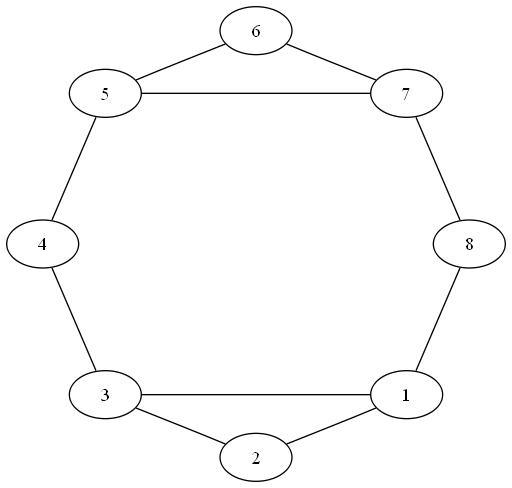
\includegraphics[width=0.5\linewidth]{./graph2.jpg}
%%\caption{}
%\label{fig:graph2}
%\end{figure}
\item State the vertices that comprise a cycle of length 5 in both of the following graphs.
%\begin{figure}[h!]
%\centering
%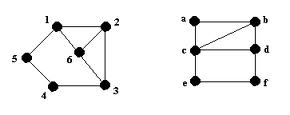
\includegraphics[width=0.7\linewidth]{./graph20.jpg}
%
%\label{fig:graph20}
%\end{figure}
\end{enumerate}



%------------------------------------%

\section*{Session 05 Graph Theory}
\begin{itemize}
\item Eulerian Path
\item Isomorphism
\item Adjacency matrices
\end{itemize}
Adjacency Matrices
\[ \left( \begin{matrix}
o & 1 & 0 & 1 & 1 \\ 
1 & 0 & 1 & 0 & 1 \\ 
1 & 1 & 0 & 1 & 1 \\ 
0 & 1 & 1 & 1 & 1 \\ 
1 & 1 & 0 & 1 & 0
\end{matrix} \right) \]


\section*{Session 05 Graph Theory}
\begin{itemize}
\item Eulerian Path
\item Isomorphism
\item Adjacency matrices
\end{itemize}
Adjacency Matrices
\[ \left( \begin{matrix}
o & 1 & 0 & 1 & 1 \\ 
1 & 0 & 1 & 0 & 1 \\ 
1 & 1 & 0 & 1 & 1 \\ 
0 & 1 & 1 & 1 & 1 \\ 
1 & 1 & 0 & 1 & 0
\end{matrix} \right) \]


%----------------------------------------------------------------%
\newpage
\section*{Condtions for Isomorphism}
\begin{itemize}
\item
\item
\item
\end{itemize}



\end{document}
